\documentclass[11pt]{article}

\pdfinfoomitdate=1
\pdftrailerid{}

\usepackage{cmap}
\usepackage[T1]{fontenc}
\usepackage{lmodern}
\usepackage[margin=1in]{geometry}
\usepackage{amsmath}
\usepackage{float}
\usepackage{graphicx}
\usepackage{microtype}
\usepackage[hidelinks]{hyperref}
\usepackage{fancyhdr}
\usepackage[
  backend=biber,
  style=numeric,
  sorting=none,
  giveninits=true,
  maxbibnames=99,
  doi=true,
  url=false,
  isbn=false
]{biblatex}

\addbibresource{refs.bib}

\hypersetup{
  pdftitle={What First-Failure Counts Miss: Admission and Downstream Fate in Ordered Validators},
  pdfauthor={Weicheng Xue},
  pdfsubject={Open technical note, version 1.0; not peer reviewed}
}

\fancypagestyle{technicalnote}{
  \fancyhf{}
  \fancyfoot[L]{\footnotesize Open technical note - version 1.0}
  \fancyfoot[R]{\footnotesize\thepage}
  \renewcommand{\headrulewidth}{0pt}
  \renewcommand{\footrulewidth}{0pt}
}
\pagestyle{technicalnote}

\begin{document}

\title{What First-Failure Counts Miss: Admission and Downstream Fate in Ordered Validators}
\author{Weicheng Xue\\[0.25em]\small\texttt{weich97}}
\date{\small Open technical note, version 1.0\\20 August 2026}

\maketitle
\thispagestyle{technicalnote}

\begin{center}
  \begin{minipage}{0.88\linewidth}
    \small
    \textbf{Publication status.}
    This document is an open technical note and has not undergone peer review.
  \end{minipage}
\end{center}

\begin{abstract}
Short-circuit validators record the first failure, a count often used to
characterize a stage's importance. We test whether that record identifies how
removing the stage changes admission or downstream behavior. For each first
hit, a scoped bypass labels the variant as newly accepted, rejected later, or
ending in an exception; a transition matrix retains later destinations. In 365
input mutations, schema validation accounts for 261 of 344 refusals (75.9\%),
yet bypassing it admits none: 250 are rejected later and 11 reach downstream
exceptions. On 24 source mutants from \texttt{idna} 3.18 selected under a
recorded outcome-blind rule, six first fail at mypy; without mypy, four pass and
two fail at pytest. First-failure counts, admission changes, and downstream fates answer
different questions and should be reported separately.
\end{abstract}

\noindent\textbf{Keywords:}
fault injection; mutation testing; validator pipelines; failure attribution;
exception exposure

\section{Introduction}

Layered validators stop at the first error, often because later checks depend
on invariants established earlier. Their trace answers where an input first
failed.

That answer is insufficient when counts guide ownership, hardening, or removal.
A frequent first hit may mask later checks; a rare one may be the last
controlled refusal before acceptance or an exception. The trace alone cannot
distinguish these outcomes. Fault-injection work has likewise argued that one
run may need more than its first observation~\cite{arlat2011collecting}.

For each mutation, we replay the first hit under a scoped bypass and record
acceptance, later rejection, exception, and any later destination. We apply the
same measurement to an artifact validator and an external Python package.

\section{Measurement and Study Design}
\label{sec:method}

For a variant $v$, let $H_i$ contain those whose first controlled rejection is
reported at unit $i$. Variants are mutated artifacts in the first case and
source mutants in the transfer. A reported unit may group path-specific checks,
but its grouping and bypass boundary must be stated.
When unit $i$ is bypassed on the applicable path, each member of $H_i$ is either
newly accepted ($C_i$), rejected by another active unit ($S_i$), or terminated
by a downstream exception ($X_i$). These outcomes give the accounting identity
\begin{equation}
  |H_i|=C_i+S_i+X_i.
  \label{eq:partition}
\end{equation}
For nonempty $H_i$, the fixed-corpus bypass fate profile is
\begin{equation}
  \mathbf{b}_i=(C_i,S_i,X_i)/|H_i|.
  \label{eq:profile}
\end{equation}
$|H_i|$ is trace provenance, $C_i$ is admission change, and $X_i$ is exception
exposure. To retain destinations hidden inside $S_i$, define
\begin{equation}
  T_{ij}=|\{v\in H_i:O_{-i}(v)=j\}|,
  \label{eq:transition}
\end{equation}
where $O_{-i}(v)$ is the outcome after bypassing unit $i$. Acceptance and
exception cells give $C_i$ and $X_i$; later-unit cells sum to $S_i$.

The first case starts from a reconciled set of JSON artifacts. Of 365 mutations, 361
alter this post-execution set and are submitted to an ordered path comprising
schema, component, binding, cross-artifact preflight, and journal validation.
The preflight repeats parts of earlier checks. Four lifecycle probes instead
call the live state machine. The
final bucket therefore joins two paths. This is mainly an offline diagnostic, not a
test of execution prevention.

The corpus contains 146 directed probes and 219 generic mutations, all authored
for this system. Each replay starts from a fresh copy of one fixed fixture. The
baseline records the first rejection or acceptance; five scoped passes then
bypass one named unit each. Here, \emph{accepted} means only that the diagnostic
path reports no validation error.

\paragraph{External-package transfer}
We then applied the accounting to the independently maintained \texttt{idna}
3.18 package. Ruff formatting, Ruff lint, strict mypy, and 6,405 collected
pytest items form an experimental projection of its upstream workflow. This
Windows sequence omits ty and all but the Python 3.12 cell, and shares no
validator, mutation generator, or tests with the first case.

Before observing outcomes, token and AST rules enumerated one-edit candidates
in the package's \texttt{core.py} module. Source-hash ordering and within-family round-robin
selection fixed 24 primary mutants: 4 layout, 4 parameter-reference, 4
annotation, 6 predicate, and 6 scalar-boundary edits. These balanced counts do
not estimate natural defect frequencies. Sixteen directed mutants calibrated
routing but do not enter the primary counts. Two controls bracketed each of two
repeats. Every mutant ran through the baseline and each single-command omission.
With no consumer after pytest, $H_i=C_i+S_i$ and $X_i$ is unavailable.

\section{Results}
\label{sec:results}

With all reported checks active, 344 variants are rejected and 21 are accepted.
The first-hit counts in reported order are 261, 20, 36, 18, and 9. Schema validation
therefore accounts for $261/344=75.9\%$ of the rejection trace.

Schema's share differs between the directed and generic strata, but the first
three admission changes remain zero within each. Figure~\ref{fig:attribution}
compares the baseline with the bypass runs. Admission changes in reported order
are 0, 0, 0, 18, and 9: the first three units produce 317 first rejections but
no new acceptance, while the last two account for all 27.

Schema bypass illustrates why admission alone is incomplete. Its fate tuple is
\begin{equation}
  (C_1,S_1,X_1)=(0,250,11).
\end{equation}
Equivalently, $\mathbf{b}_1=(0,95.8\%,4.2\%)$. Of the later rejections, 246 move
to component validation and four to preflight; the other 11 reach code whose
shape or type assumptions no longer hold. Component bypass sends six first hits
to binding and 14 to preflight, while binding bypass sends all 36 to preflight.

\begin{figure}[H]
  \centering
  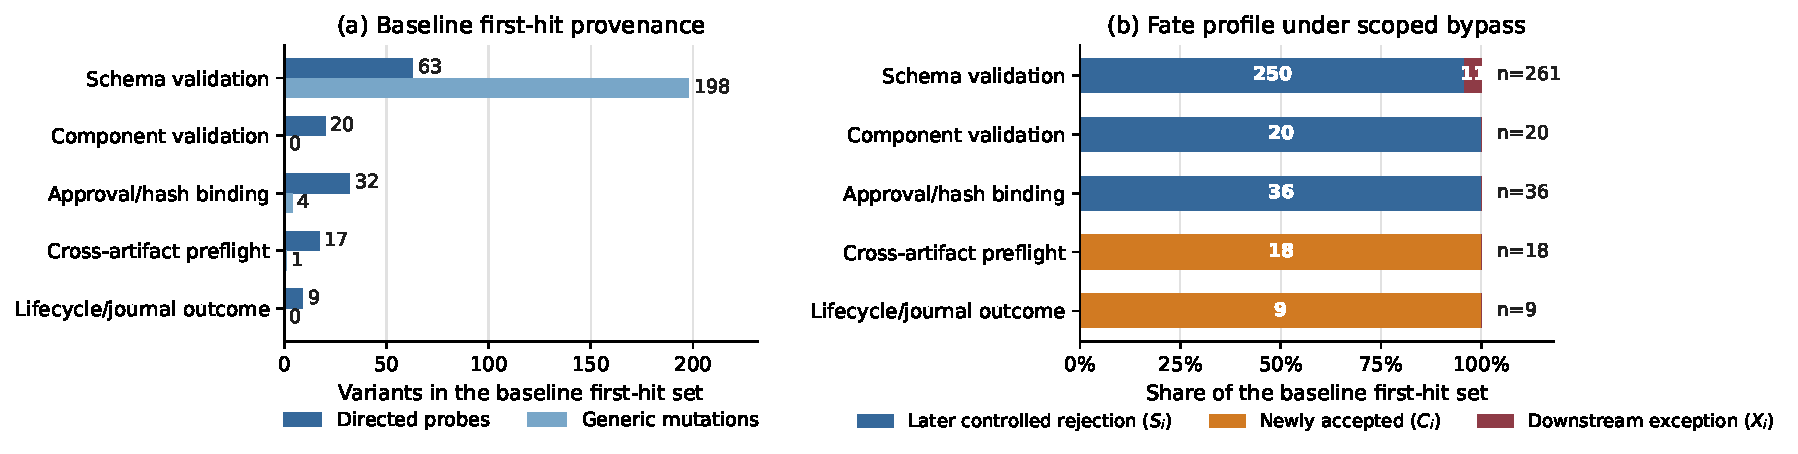
\includegraphics[width=\linewidth]{figures/attribution_gap.pdf}
  \caption{Baseline first-hit provenance by mutation source (a) and the scoped
  bypass fate profile (b).}
  \label{fig:attribution}
\end{figure}

\begin{table}[H]
  \centering
  \small
  \caption{External-package first hits ($H$) and scoped-omission fates. Five
  other primary mutants pass the chain; $X$ is unavailable after pytest.}
  \label{tab:external}
  \begin{tabular}{lrrrl}
    \hline
    Command & $H$ & $C$ & $S$ & Later destination \\
    \hline
    Ruff format & 4 & 4 & 0 & -- \\
    Ruff lint & 0 & 0 & 0 & -- \\
    mypy & 6 & 4 & 2 & pytest (2) \\
    pytest & 9 & 9 & 0 & -- \\
    \hline
  \end{tabular}
\end{table}

\paragraph{External-package transfer}
The two repeats agreed. Five primary mutants passed the chain. Among the six
that first failed at mypy, all four annotation edits passed when mypy was
omitted, while both parameter-reference edits failed at pytest. One first-hit
bucket therefore contained admission changes and later rejections. Its pooled
four-of-six rate depends on the fixed family mix. Ruff lint's zero is likewise
specific to this corpus, not an estimate of lint utility.

\section{Implications and Limitations}
\label{sec:discussion}

The first-hit count locates the earliest refusal, the fate profile records what
the stated bypass admits or exposes, and the transition matrix shows where
later refusals move. None is a stage ranking. A stage with $C_i=0$ may still
improve diagnostics, and a terminal stage has no downstream substitute.

The estimand follows the intervention: the artifact case bypasses call sites,
whereas \texttt{idna} omits whole commands. Both use deterministic replay and a
clean reset, but at different granularities. The artifact result concerns one
fixture, authored mutations, and a mostly post-execution diagnostic; its final
bucket also combines two paths. A later refusal does not establish an
independent implementation of the same rule.

The external package is independently maintained, but the experiment is ours.
Its 24 balanced mutants and Windows sequence do not represent natural defects
or the full upstream workflow. Passing means only that this sequence accepted a
mutant. With terminal pytest, exception exposure is unavailable in this case.
The released plan and catalog record the outcome-blind selection rule, but the
selector implementation is not included; this release therefore audits the
record rather than regenerating the selection.

The first transfer run stopped at a pytest reporting timeout. A diagnostic
revealed that cell's pytest fate; we then changed only failure rendering and
evidence capture and reran the unchanged catalog, order, and analysis from the
first control. That one outcome was therefore known before the final run.

\section{Related Work}

Fault injection evaluates detection and recovery under controlled
perturbations~\cite{hsueh1997faultinjection}. Mutation testing supplies the
broader vocabulary~\cite{jia2011mutation}, but mutants are not perfect
substitutes for real faults~\cite{just2014mutants}, and conclusions from
software fault injection depend on fault-load representativeness
~\cite{natella2013representativeness}.

Arlat and Moraes argue for retaining multiple observations from a fault-
injection run rather than relying on its first event
~\cite{arlat2011collecting}. Steininger evaluates combinations of error-
detection mechanisms from fault-injection results
~\cite{steininger2002identifying}. We operationalize these ideas for
short-circuit software validators by assigning every first-hit input to an
acceptance, later-rejection, or exception fate under a scoped intervention.

Recent mutation studies distinguish kill mechanisms, including crashes
~\cite{du2023kill}, and separate state infection, propagation, and observable
failure~\cite{du2024ripples}. Causal Testing changes executions to distinguish
root causes from coincident features~\cite{johnson2020causal}. Our transition
matrix applies the same intervention logic to the ordered destinations of
validator refusals.

\section{Conclusion}

First-failure counts tell us where validation stopped, not how omitting a stage
changes admission or downstream fate. Schema was first for 75.9\% of refusals
in the artifact case, yet its bypass admitted nothing: 250 mutations failed
later and 11 ended in exceptions. In \texttt{idna}, omitting mypy admitted four of six first
hits while two moved to pytest. Across both cases, decisions about hardening or
removing a stage require admission and downstream fate as well as first-failure
provenance.

\clearpage
\printbibliography

\end{document}
